\documentclass[12pt,a4paper]{article}

% Paquetes básicos
\usepackage[utf8]{inputenc}
\usepackage[T1]{fontenc}
\usepackage[english]{babel}
\usepackage{amsmath, amssymb}
\usepackage{siunitx} 
\usepackage{graphicx}
\usepackage{float}
\usepackage{geometry}
\usepackage{xcolor}
\geometry{margin=2.5cm}
\usepackage{hyperref}
\usepackage{caption}
\usepackage{subcaption}
\usepackage{setspace}
\usepackage{multirow}
\usepackage{minted}  
\usepackage{gensymb} 
%\usepackage[backend=biber, style=ieee]{biblatex}
\usepackage[american, straightvoltages]{circuitikz}
\usepackage{csquotes}
\usepackage{indentfirst}
%\addbibresource{references.bib}

\graphicspath{{Figures/}}
\onehalfspacing
\hypersetup{
    colorlinks  = true,
    linkcolor   = blue,    
    citecolor   = blue,
    urlcolor    = blue,
    filecolor   = blue
}

\begin{document}       
\renewcommand{\figureautorefname}{Fig.}
\renewcommand{\tableautorefname}{Tab.}
\renewcommand{\equationautorefname}{Eq.}


% Carátula personalizada
\begin{titlepage}
    \centering
    
\includegraphics[width=0.7\textwidth]{Fulgor Logo.png}\\[1.5cm]

    {\Large \textbf{FUNDACIÓN FULGOR} \\[0.5cm]}
    {\Large CMOS Course} \\[0.5cm]

    \rule{\textwidth}{0.5pt} \\[0.5cm]
    {\Large \textbf{Homework N°3} \\[0.3cm]}
    \rule{\textwidth}{0.5pt} \\[1cm]
    
\begin{tabular}{l l}
    \textbf{Professors:} & Michel Saenz.\\
                         & Santiago Castro.\\
    \\
    \textbf{Student:}    & Monja, Ernesto Joaquín (43.873.728)\\
\end{tabular} \\[5cm]

{\centering Year 2026 \par}

\end{titlepage}



% Índice
\tableofcontents
\newpage



\section{Introduction}                                          \label{sec_1}
This report analyzes the \textit{DC} operating point and transient response of a \textit{Common Source CMOS} amplifier with Biasing shown in \autoref{fig:fig_1}. 
\begin{figure}[H]
    \centering
    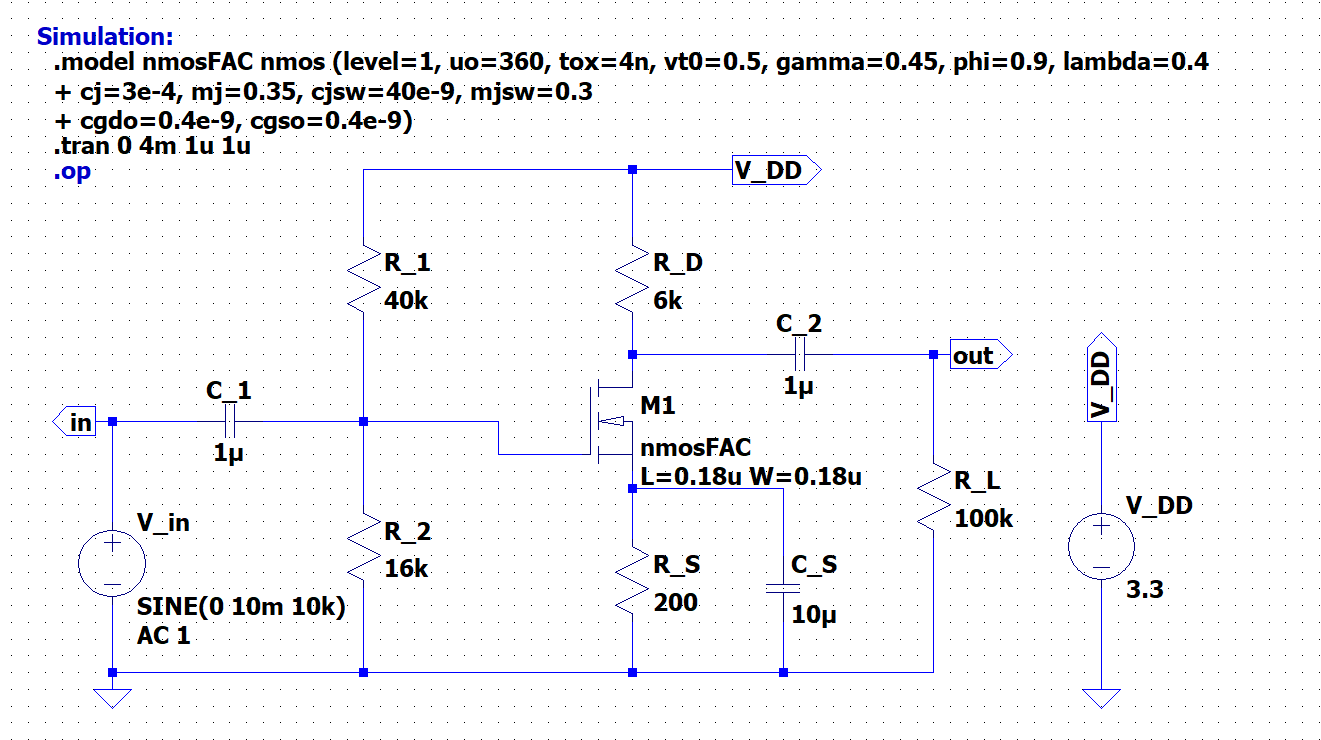
\includegraphics[width=0.85\linewidth]{Figure 1.png}
    \caption{Circuit proposed to analyze.} 
    \label{fig:fig_1}
\end{figure}

Using the provided $W = L = 0.18 \ [\mu m]$ \textit{CMOS} model, theoretical hand calculations are compared with \textit{LTspice} simulations to verify proper saturation bias and evaluate the dynamic mid-band voltage gain.



\section{DC Operating Point Analysis}                           \label{sec_2}
The objective of this section is to ensure the \textit{MOSFET} is properly biased in the saturation region (linear amplification zone) using the provided \textit{nmosFAC} model for $W = L = 0.18 \ [\mu m]$. 


\subsection{Theoretical Calculations}                           \label{sec_2.1}
Assuming the gate current is negligible ($I_{G} = 0$), the gate voltage $V_{G}$ is determined by the resistive voltage divider formed by $R_2$ and $R_3$:
\begin{equation}
    V_{G} = \frac{V_{DD} \cdot R_{2}}{R_{1} + R_{2}} = \frac{3.3 \cdot 16k}{16k + 40k} \approx 0.9429 \, [V]
    \label{eq_1}
\end{equation}

Based on the \textit{CMOS} model for the transistor provided shown below:
\begin{minted}[linenos]{bash}
.model nmosFAC nmos (level=1, uo=360, tox=4n, vt0=0.5, gamma=0.45, phi=0.9, 
                    + lambda=0.4, cj=3e-4, mj=0.35, cjsw=40e-9, mjsw=0.3
                    + cgdo=0.4e-9, cgso=0.4e-9)
\end{minted}

We can see that the threshold voltage is equal to: $V_{Th0} = 0.5 \, [V]$. Therefore, the source voltage $V_{S}$ depends on the drain current $I_{D}$ and the source degradation resistor $R_{S}$:
\begin{equation}
    V_{S} = I_{D} \cdot R_{S} = I_D \cdot (200)
    \label{eq_2}
\end{equation}

For the transistor to be turned on, the gate-source voltage must exceed the threshold voltage, this is: $V_{GS} = V_{G} - V_{S} > V_{Th}$. The drain current in saturation (ignoring channel-length modulation, this is: $\lambda = 0$ for the initial hand-calculation estimate) is given by:
\begin{equation}
    I_{D} = \frac{1}{2} \mu_{n} C_{ox} \frac{W}{L} ((V_{G} - V_{S}) - V_{Th0})^{2}
    \label{eq_3}
\end{equation}

Replacing in \autoref{eq_3} the value for $V_{Th0}$ and the one for $V_{G}$ obtained in \autoref{eq_1}, we have:
\begin{equation}
    I_{D} = \frac{1}{2} \mu_{n} C_{ox} \frac{W}{L} (0.9429 - I_D(200) - 0.5)^{2}
    \label{eq_4}
\end{equation}

From the \textit{CMOS} model, we can also note that the oxide thickness is $t_{ox} = 4 \, [nm]$. Then, we know that the value of $C_{ox}$ is given by \autoref{eq_5}.
\begin{equation}
    C_{ox} = \frac{\epsilon_{ox}}{t_{ox}}
    \label{eq_5}
\end{equation}

\noindent
where $\epsilon_{ox}$ is the relative permittivity of $SiO_{2}$ and is equal to:
\begin{equation}
    \epsilon_{ox} = \epsilon_{r} \cdot \epsilon_{0} = 3.9 \cdot 8.854x10^{-14} \approx 3.453x10^{-13} \, \left[\frac{F}{cm}\right]
    \label{eq_6}
\end{equation}

Therefore, we have that combining \autoref{eq_5} and \autoref{eq_6}, we have:
\begin{equation}
    C_{ox} = \frac{3.453x10^{-13} \, \left[\frac{F}{cm}\right]}{4x10^{-7} \, [cm]} \approx 8.63x10^{-7} \, \left[\frac{F}{cm^{2}} \right]
    \label{eq_7}
\end{equation}

Given that the electron mobility is equal to: $\mu_{n} = 360 \, [\frac{cm^{2}}{Vs}]$ and that the \textit{CMOS} model has a: $W = L = 0.18 \ [\mu m]$, we can replace these values and the one obtained in \autoref{eq_7}, into \autoref{eq_4} (recall that we are initially ignoring channel-length modulation, this is: $\lambda = 0$), so that we have:
\begin{equation}
    I_{D} = \frac{1}{2} \cdot \left(360 \, \frac{cm^{2}}{Vs}\right) \cdot \left(8.63x10^{-7} \, \frac{F}{cm^{2}}\right) \cdot \left(\frac{0.18 \, \mu m}{0.18 \, \mu m}\right) \cdot (0.4429 - 200 \cdot I_{D})^{2}
    \label{eq_8}
\end{equation}
\begin{equation}
    I_{D} \approx 155.34x10^{-6}(0.4429^{2} - 2 \cdot 0.4429 \cdot 200 \cdot I_D + 40000 \cdot I_D^2)
    \label{eq_9}
\end{equation}
\begin{equation}
    I_{D} = 30.48x10^{-6} - 0.02753 \cdot I_{D} + 6.216 \cdot I_{D}^{2}
    \label{eq_10}
\end{equation}

Rearranging the expression obtained in \autoref{eq_10} into the standard quadratic form:
\begin{equation}
    6.216 \cdot I_{D}^{2} - 1.02753 \cdot I_{D} + 30.48x10^{-6} = 0
    \label{eq_11}
\end{equation}

Now we can solve for $I_{D}$ using the quadratic formula, where we obtain the following two solutions:
\begin{equation}
    \begin{cases}
        I_{D1} = 0.1652 \, [A]\\
        I_{D2} = 29.668 \, [\mu A]
    \end{cases}
    \label{eq_12}
\end{equation}

We note that from \autoref{eq_12} that we have two possible solutions for $I_{D}$ yet only the smaller value is physically valid. The larger root would result in an excessive voltage drop across the source resistor ($R_{S}$), forcing the gate-source voltage ($V_{GS}$) below the threshold voltage ($V_{Th}$) and violating the active conduction assumption. Therefore, the lower current value is strictly chosen to satisfy the physical turn-on condition $V_{GS} > V_{Th}$.

Now, with the drain current established, the preliminary drain-source voltage $V_{DS}$ is:
\begin{equation}
    V_{DS} = V_{DD} - I_{D} \cdot (R_{D} + R_{S}) = 3.3 - 29.668\mu \cdot (6200) \approx 3.116 \, [V]
    \label{eq_13}
\end{equation}

Notice that the provided physical parameters describe a short-channel device and even the model for the \textit{CMOS} transistor includes a non zero channel-length modulation parameter (this is: $\lambda = 0.4$) which significantly increases the current. If we apply the corresponding correction factor, we have:
\begin{equation}
    I_{D; \, real} = I_{D} \cdot (1 + \lambda \cdot V_{DS}) = 29.668x10^{-6} \cdot (1 + 0.4 \cdot 3.116) \approx 66.64 \, [\mu A]
    \label{eq_14}
\end{equation}

Finally, we recalculate the true \textit{DC} drain-source voltage using the corrected current:
\begin{equation}
    V_{DS; \, real} = V_{DD} - I_{D; \, real} \cdot (R_{D} + R_{S}) = 3.3 - 66.64x10^{-6}(6200) \approx 2.886 \, [V]
    \label{eq_15}
\end{equation}



\subsection{\textit{LTspice} Simulation Results}                \label{sec_2.2}
The circuit was implemented in \textit{LTspice} using the \textit{CMOS} model given. A \textit{DC} operating point simulation was executed using the \texttt{.op} directive where we obtained he following results:
\begin{figure}[H]
    \centering
    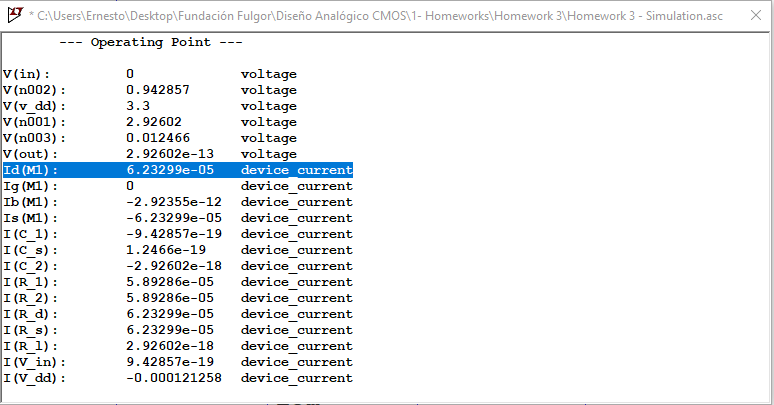
\includegraphics[width=0.8\linewidth]{Figure 2.png}
    \caption{Results of \texttt{.op} simulation in \textit{LTspice}}
    \label{fig:fig_2}
\end{figure}

With the results calculated in \autoref{eq_1}, \autoref{eq_14}, \autoref{eq_15} and the results given by the simulation in \autoref{fig:fig_2}, we can make a comparison table of the simulation versus calculation results:
\begin{table}[H]
    \centering
    \begin{tabular}{|c|c|c|} \hline
    \textbf{Parameter} & \textbf{Theoretical Estimate} & \textbf{LTspice Simulation} \\ \hline
    $V_{G}$     & $0.9429 \, [V]$       & $0.942857 \, [V]$     \\ \hline
    $I_{D}$     & $66.64 \, [\mu A]$    & $62.3299 \, [\mu A]$  \\ \hline
    $V_{DS}$    & $2.886 \, [V]$        & $2.913554 \, [V]$     \\ \hline
    \end{tabular}
    \caption{Comparison of theoretical hand calculations and \textit{LTspice DC} simulation.}
    \label{tab:tab_1}
\end{table}

We can see that the values calculated are practically identical to the ones simulated, therefore validating the model and the equations used in the \autoref{sec_2.1}. Note that the small discrepancies between theoretical and simulated values are mainly attributed to the body effect ($\gamma$) not being manually calculated, which slightly increases the threshold voltage as $V_{S} > 0$ that we can verify as $V_{S} \approx 12.46 \, [mV]$ in \autoref{fig:fig_2}.



\section{Transient Response (Time-Domain Analysis)}             \label{sec_3}    
The objective of this phase is to evaluate the dynamic processing and amplification of a small, time-varying signal.


\subsection{Simulation Setup}                                   \label{sec_3.1}
\begin{itemize}
    \item \textbf{Source Configuration:} The input voltage source ($V_{in}$) was configured as a sine wave (\texttt{SINE}) with no \textit{DC} offset, a peak amplitude of $10 \, [mV]$, and a frequency of $10 \, [kHz]$.
    \item \textbf{Transient Analysis:} The simulation was executed using the \texttt{.tran 0 4m 1u 1u} command. Because the period of a $10 \, [kHz]$ signal is $0.1 \, [ms]$, a $4 \, [ms]$ simulation time captures several complete cycles to properly observe the steady-state dynamic behavior.
\end{itemize}


\subsection{Measurements and Voltage Gain}                      \label{sec_3.2}
Both the input signal at the gate and the amplified output signal were plotted simultaneously and we can see the results of this simulation in \autoref{fig:fig_3}.
\begin{figure}[H]
    \centering
    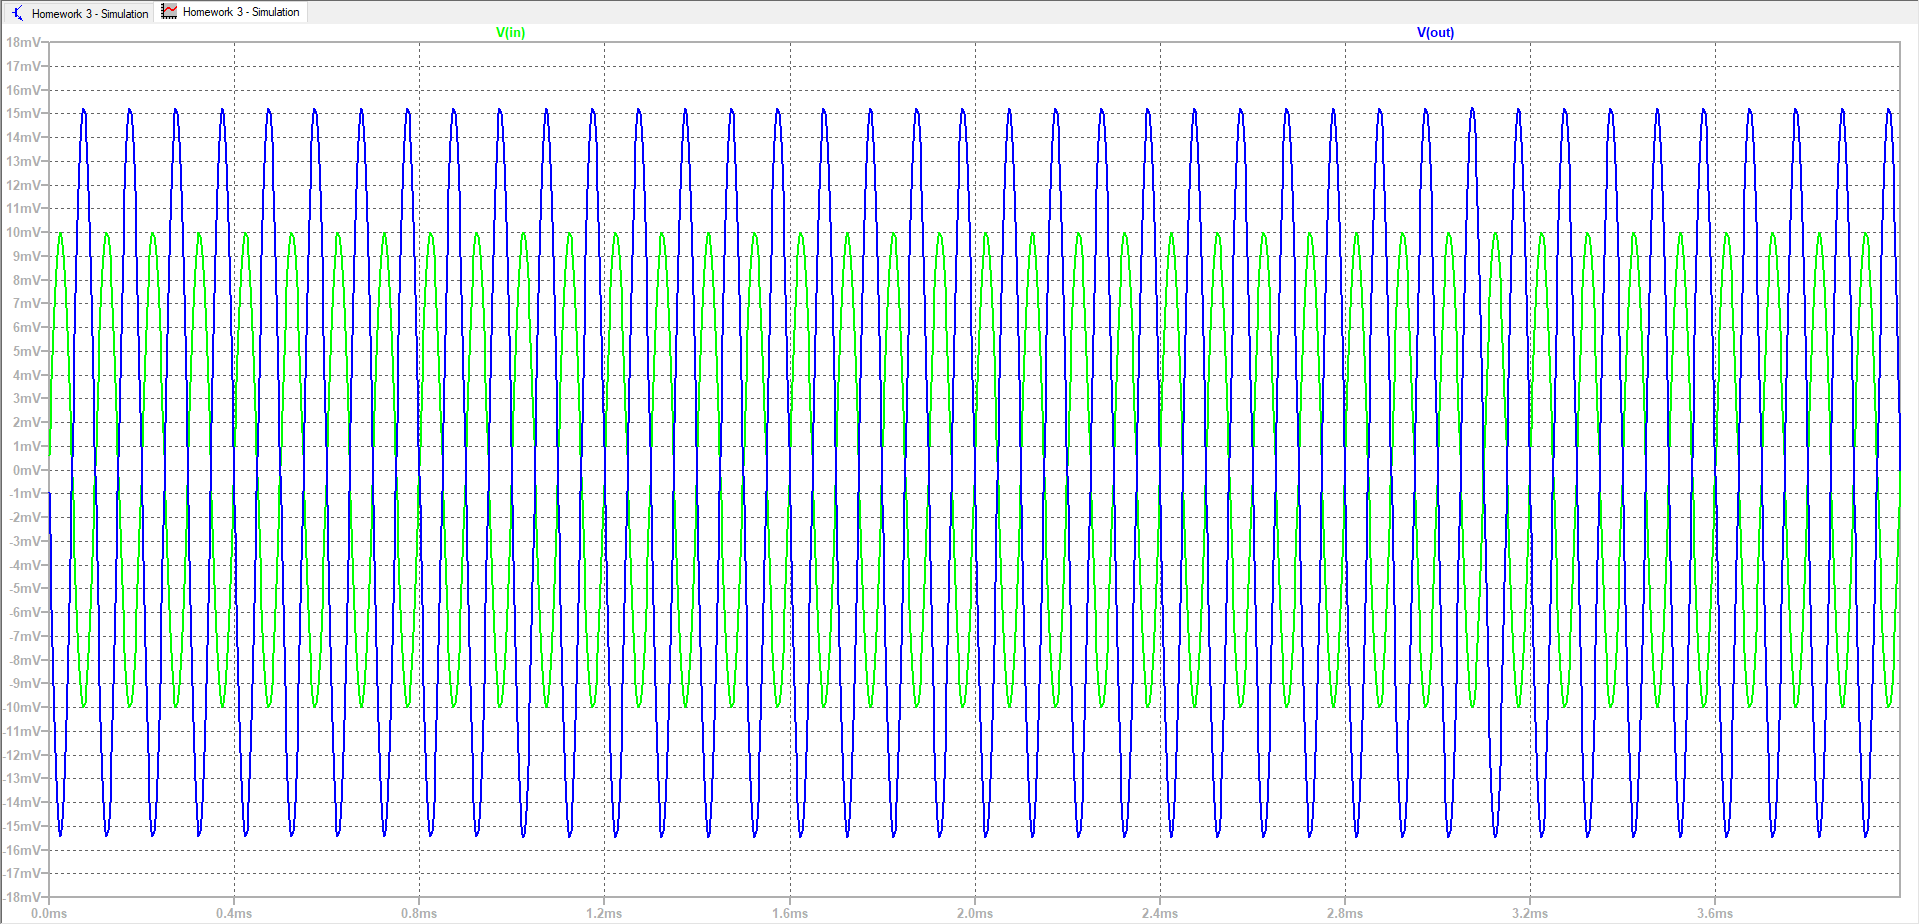
\includegraphics[width=1\linewidth]{Figure 3.png}
    \caption{Results of \texttt{.tran} simulation in \textit{LTspice}, where we see in \color{green}{green} \color{black}{the input voltage ($v_{in}$) and in} \color{blue}{blue} \color{black}{the output voltage ($v_{out}$).}}
    \label{fig:fig_3}
\end{figure}

We can see from the y-axis, that:
\begin{itemize}
    \item Input peak-to-peak voltage: $V_{in,pp} = 20 \, [mV]$
    \item Output peak-to-peak voltage: $V_{out,pp} = 30 \, [mV]$
\end{itemize}

Therefore, the mid-band voltage gain ($A_{v}$) of the amplifier is calculated as the ratio of the output to the input peak-to-peak voltage, this is:
\begin{equation}
    A_v = \frac{V_{out,pp}}{V_{in,pp}} = \frac{30 \, [mV]}{20 \, [mV]} = 1.5 \, \left[\frac{V}{V} \right]
    \label{eq_16}
\end{equation}

Note that the result obtained in \autoref{eq_16} shows an exceptionally low simulated mid-band voltage gain. This is not an error but rather a direct consequence of the dimensions of the device (where $W = L = 0.18 \, [\mu m]$): An aspect ratio of $W/L = 1$ restricts the drain current to approximately $62 \, [\mu A]$, severely limiting the transconductance ($g_{m}$) and since the voltage gain is proportional to $g_{m}$, the amplifier cannot provide significant amplification under these sizing constraints.



\section{Conclusion}                                            \label{sec_4}
This report analyzed the \textit{DC} operating point and transient response of a Common Source \textit{CMOS} amplifier. The \autoref{sec_2} demonstrated that theoretical calculations, especially when including the channel-length modulation parameter ($\lambda$), closely match the \textit{LTspice} simulations; where as \autoref{sec_3} confirmed a proper linear operation but revealed a marginal voltage gain ($1.5 \, [V/V]$). This highlights a key principle in analog \textit{CMOS} design: while correct \textit{DC} biasing is necessary, proper device sizing ($W/L$) is strictly required to achieve the desired amplification.

%\newpage
%\printbibliography[heading=bibintoc, title={4 \, \, Bibliography}]
\end{document}